% Ubah judul dan label berikut sesuai dengan yang diinginkan.
\section{Result}
\label{sec:results}
 
The metrics employed to assess the efficacy of the model during training are accuracy and loss. These two metrics are utilized to ascertain the suitability of the model for the task at hand. However, they may prove challenging in predicting data that has never been encountered by the model.

The testing process involves three models, namely the model with the highest training accuracy value, the model with the highest validation value, and the last model in training.

The results of this study were evaluated using several additional metrics, including precision, recall, and F1-score. These metrics are employed to assess the accuracy of the model that has been developed.
\subsection{Model Testing Results Without Using class-weight Adjustment}
\begin{figure}[hbtp]
	\centering
	\subfloat[\centering Training Loss dan Akurasi ResNet-18]{{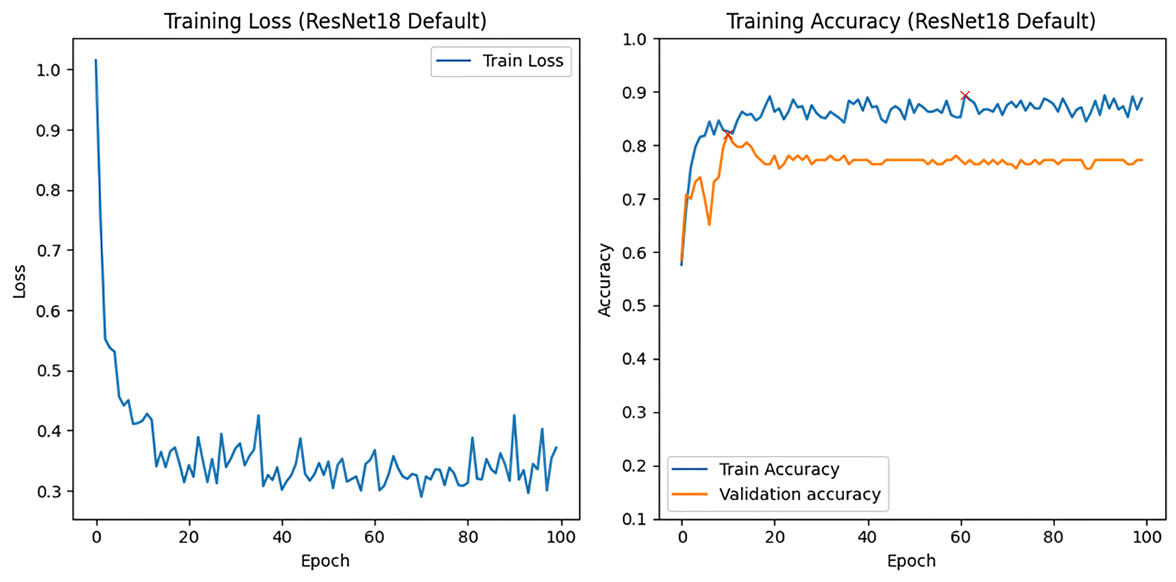
\includegraphics[height=4cm]{gambar/TrainingGraphResNet18.png}}}
	\qquad
	\subfloat[\centering Training Loss dan Akurasi ResNet-34]{{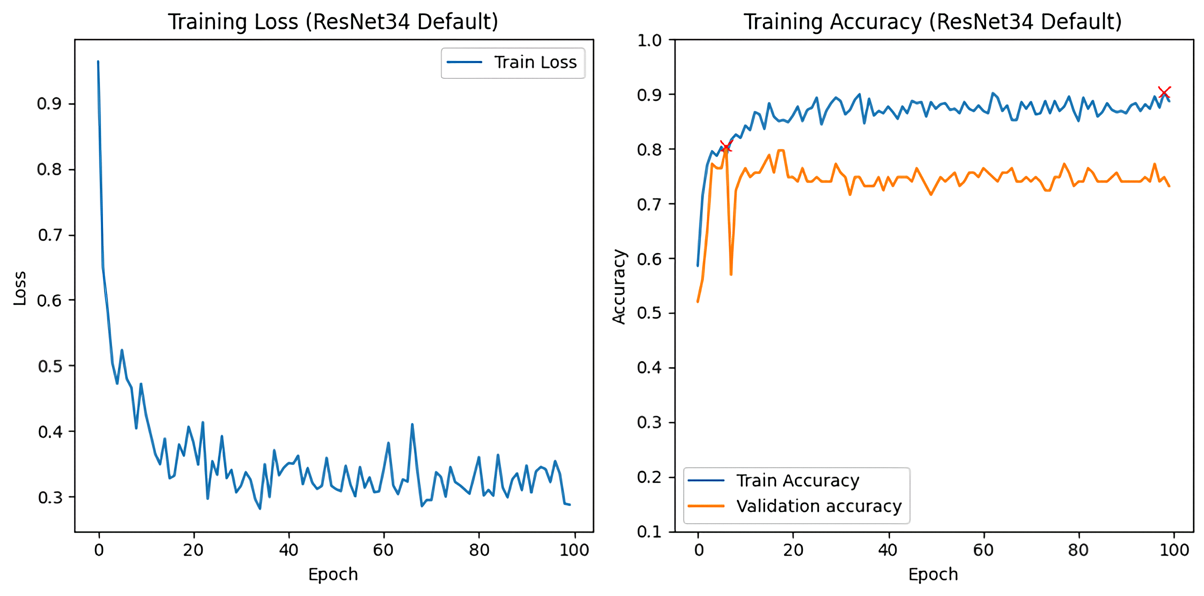
\includegraphics[height=4cm]{gambar/TrainingGraphResNet34.png}}}
	\caption{Grafik Training Loss dan akurasi ResNet-18 dan ResNet-34 Tanpa Penyesuaian Beban pada \emph{Class}}
	\label{Fig:GraphTrainingDefPt1}
\end{figure}

\begin{figure}[hbtp]
	\centering
	\subfloat[\centering Training Loss dan Akurasi ResNet-50]{{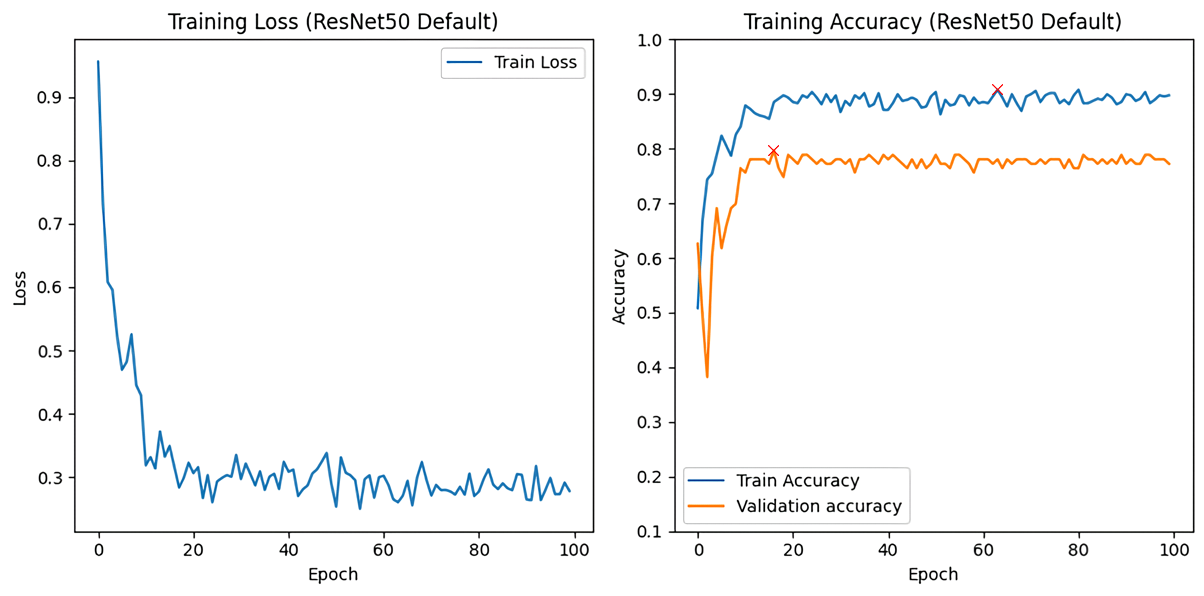
\includegraphics[height=4cm]{gambar/TrainingGraphResNet50.png}}}
	\qquad
	\subfloat[\centering Training Loss dan Akurasi ResNet-101]{{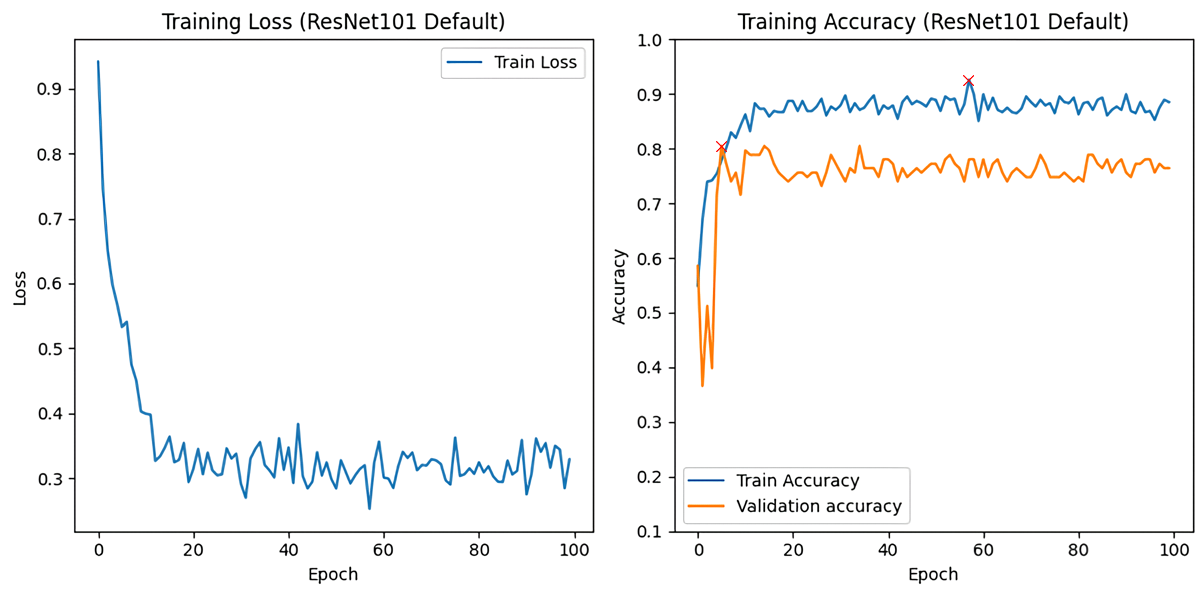
\includegraphics[height=4cm]{gambar/TrainingGraphResNet101.png}}}
	\caption{Grafik Training Loss dan akurasi ResNet-50 dan ResNet-101 Tanpa Penyesuaian Beban pada \emph{Class}}
	\label{Fig:GraphTrainingDefPt2}
\end{figure}

\begin{figure}[hbtp]
	\subfloat[\centering Training Loss dan Akurasi ResNet-152]{{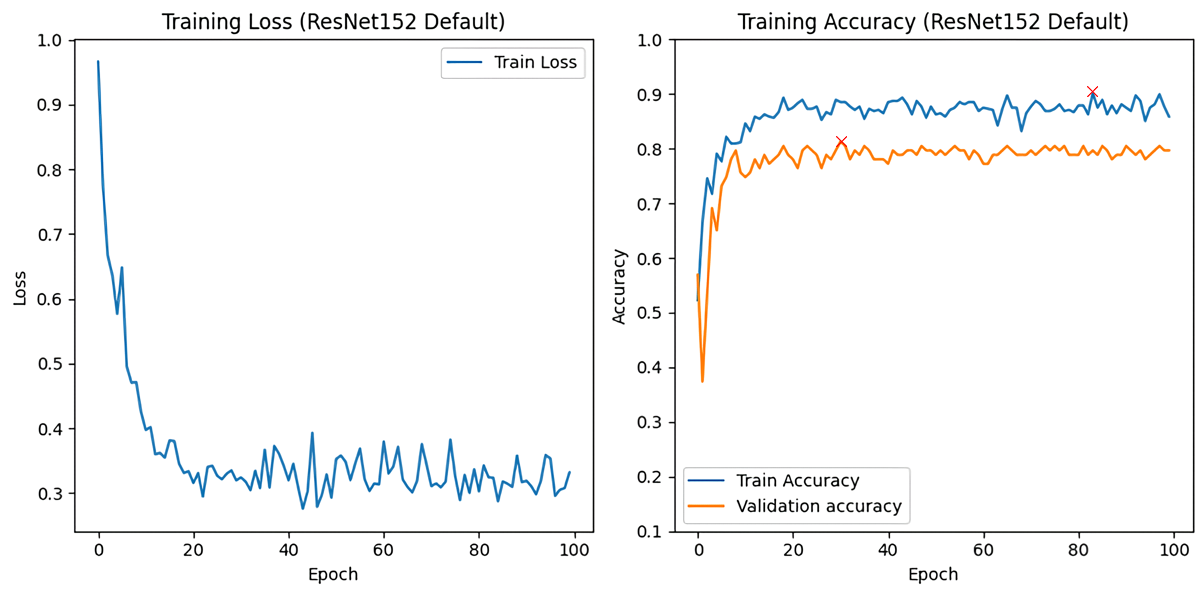
\includegraphics[height=4cm]{gambar/TrainingGraphResNet152.png}}}
	\caption{Grafik Training Loss dan akurasi ResNet-152 Tanpa Penyesuaian Beban pada \emph{Class}}
	\label{Fig:GraphTrainingDefPt3}
\end{figure}

\subsection{Model Testing Results Using class-weight Adjustment}
\label{sec:412}
\begin{figure}[hbtp]
	\centering
	\subfloat[\centering Training Loss dan akurasi ResNet-18]{{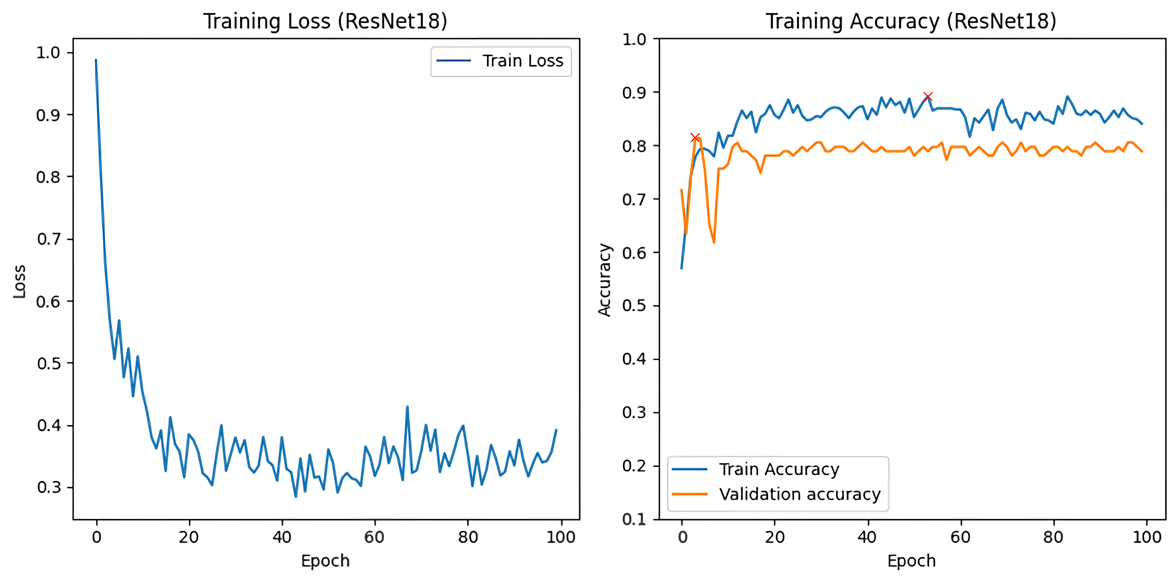
\includegraphics[height=4cm]{gambar/TrainingGraphResNet18class-weighted.png}}}
	\qquad
	\subfloat[\centering Training Loss dan akurasi ResNet-34]{{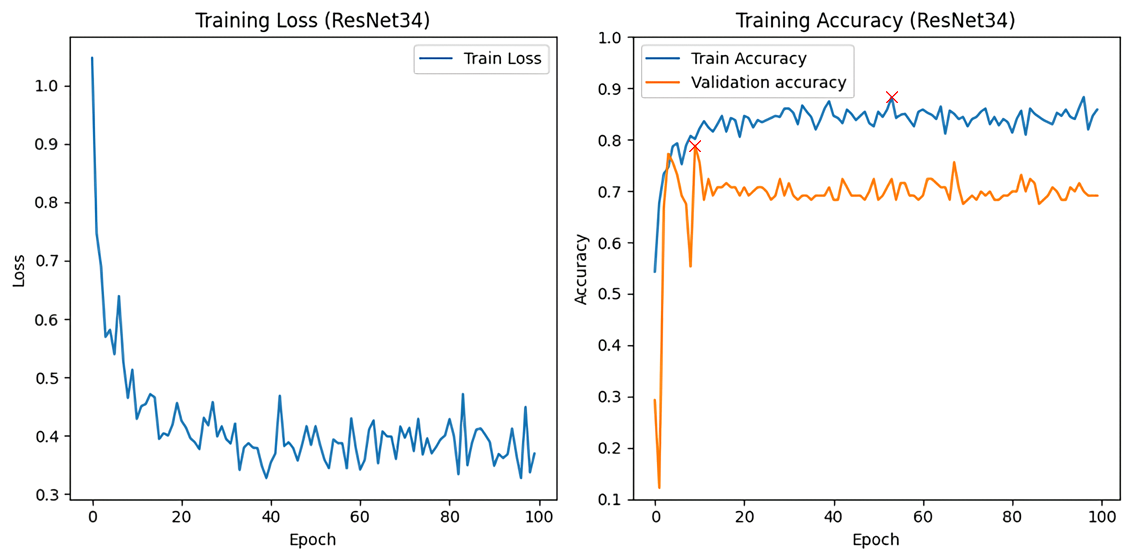
\includegraphics[height=4cm]{gambar/TrainingGraphResNet34class-weighted.png}}}
	\caption{Grafik Training Loss dan akurasi ResNet-18 dan ResNet-34 dengan Penyesuaian Beban pada \emph{Class}}
	\label{fig:graphTrainingWeightedPt1}
\end{figure}

\begin{figure}[hbtp]
	\centering
	\subfloat[\centering Training Loss dan akurasi ResNet-50]{{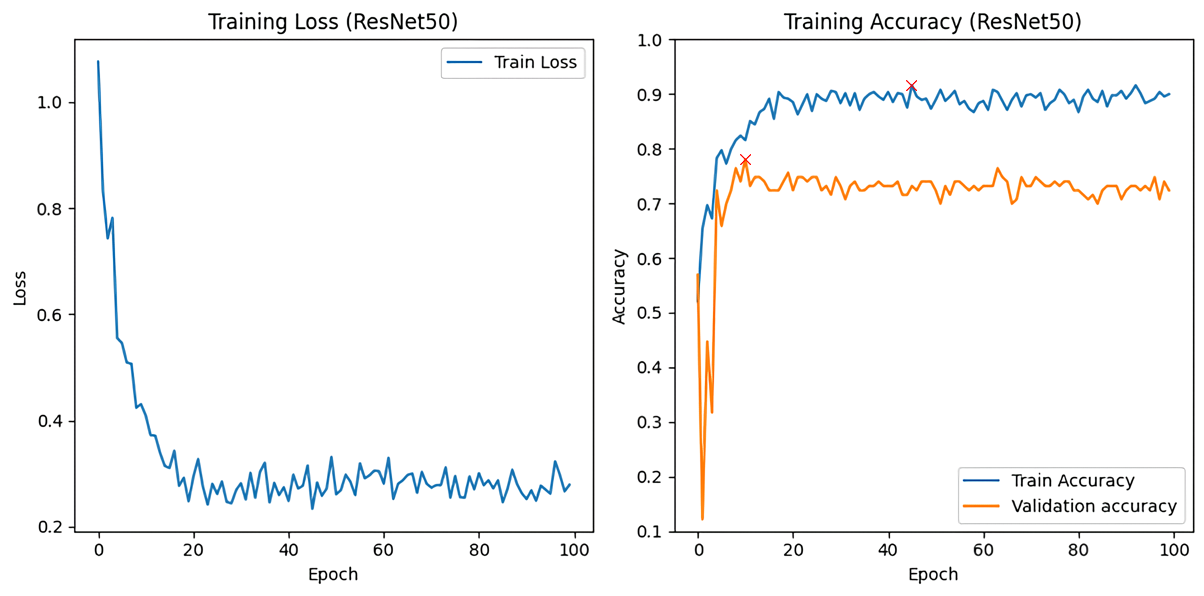
\includegraphics[height=4cm]{gambar/TrainingGraphResNet50class-weighted.png}}}
	\qquad
	\subfloat[\centering Training Loss dan akurasi ResNet-101]{{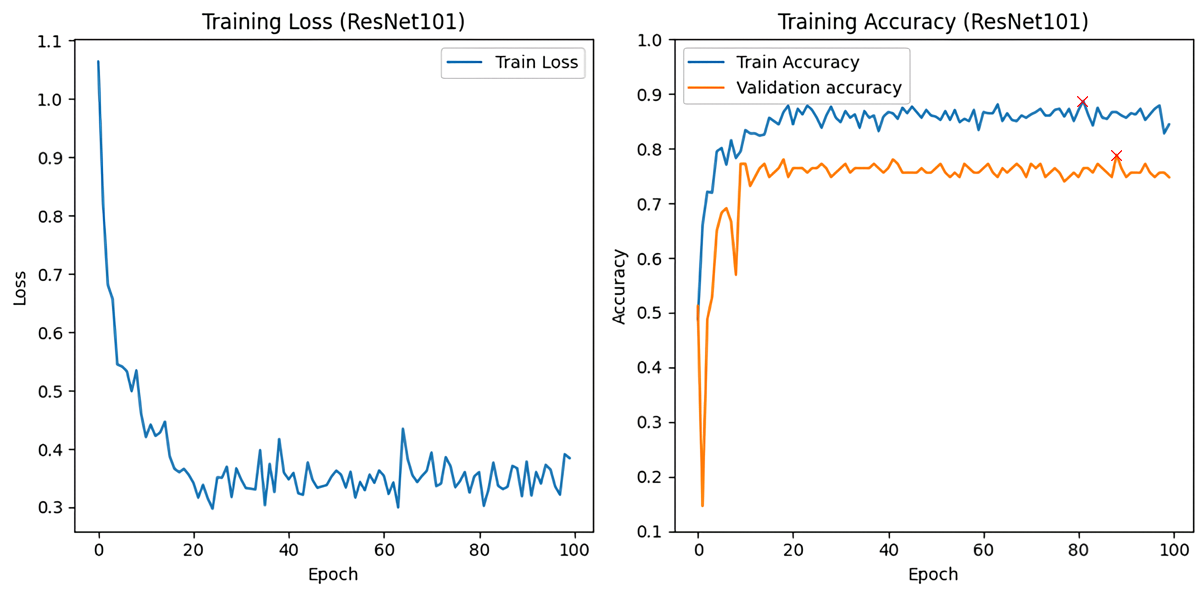
\includegraphics[height=4cm]{gambar/TrainingGraphResNet101class-weighted.png}}}
	\caption{Grafik Training Loss dan akurasi ResNet-50, 101 dengan Penyesuaian Beban pada \emph{Class}}
	\label{fig:graphTrainingWeightedPt2}
\end{figure}

\begin{figure}[hbtp]
	\centering
	\subfloat[\centering Training Loss dan akurasi ResNet-152]{{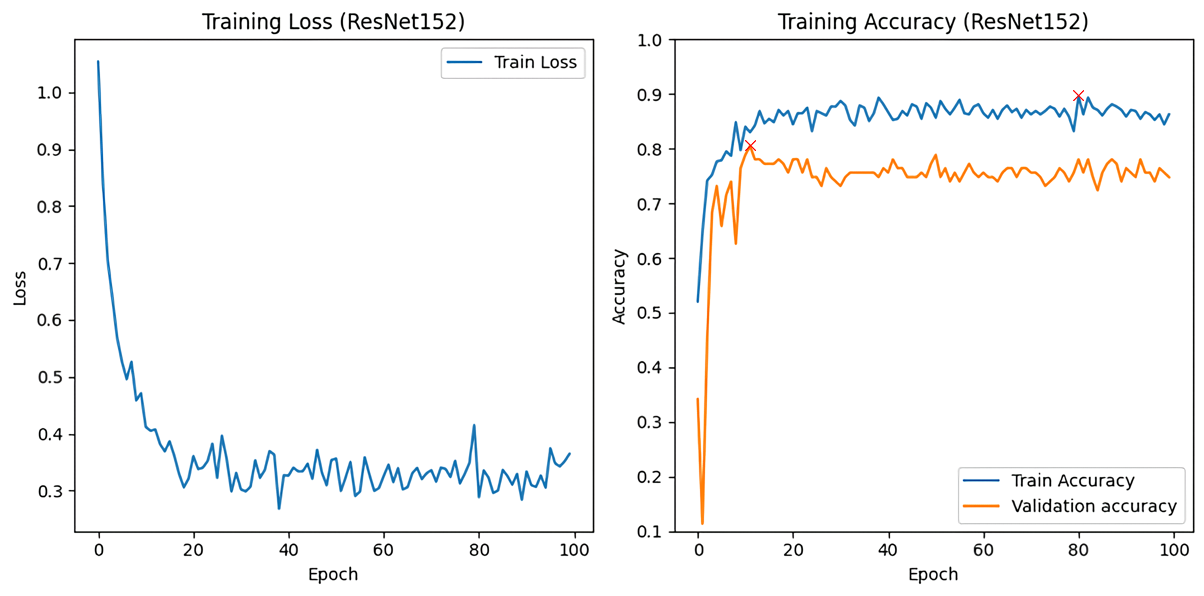
\includegraphics[height=4cm]{gambar/TrainingGraphResNet152class-weighted.png}}}
	\caption{Grafik Training Loss dan akurasi ResNet-152 dengan Penyesuaian Beban pada \emph{Class}}
	\label{fig:graphTrainingWeightedPt3}
\end{figure}

\begin{table}[hbtp]
	\begin{center}
	\caption{Perbandingan Nilai Akurasi, Recall pada class PDR. dan QWK dari setiap \emph{Best Trained Model} dengan Pembebanan pada \emph{Class} dan tanpa Pembebanan pada \emph{Class}}
	\label{tb:PerbandinganHasilBestTrain}
	\begin{tabular}{|c|c|lll|ccc|}
		\hline
		\cellcolor[HTML]{C0C0C0}                             & \cellcolor[HTML]{C0C0C0}                                  & \multicolumn{3}{c|}{\cellcolor[HTML]{C0C0C0}Akurasi Metrik}                           & \multicolumn{3}{c|}{\cellcolor[HTML]{C0C0C0}Selisih}                                                                            \\ \cline{3-8} 
		\multirow{-2}{*}{\cellcolor[HTML]{C0C0C0}Arsitektur} & \multirow{-2}{*}{\cellcolor[HTML]{C0C0C0}Metode training} & \multicolumn{1}{c|}{Overall} & \multicolumn{1}{c|}{PDR}    & \multicolumn{1}{c|}{QWK} & \multicolumn{1}{c|}{Overall}                   & \multicolumn{1}{c|}{PDR}                        & QWK                          \\ \hline
															 & Default                                                   & \multicolumn{1}{l|}{0,7642}  & \multicolumn{1}{l|}{0,5}    & 0,7584                   & \multicolumn{1}{c|}{}                          & \multicolumn{1}{c|}{}                           &                              \\ \cline{2-5}
		\multirow{-2}{*}{ResNet-18}                          & \multicolumn{1}{l|}{Class-Weighted}                       & \multicolumn{1}{l|}{0,7886}  & \multicolumn{1}{l|}{0,7143} & 0,7527                   & \multicolumn{1}{c|}{\multirow{-2}{*}{0,0244}}  & \multicolumn{1}{c|}{\multirow{-2}{*}{0,214286}} & \multirow{-2}{*}{-0,005667}  \\ \hline
															 & Default                                                   & \multicolumn{1}{l|}{0,748}   & \multicolumn{1}{l|}{0,5714} & 0,7218                   & \multicolumn{1}{c|}{}                          & \multicolumn{1}{c|}{}                           &                              \\ \cline{2-5}
		\multirow{-2}{*}{ResNet-34}                          & \multicolumn{1}{l|}{Class-Weighted}                       & \multicolumn{1}{l|}{0,7236}  & \multicolumn{1}{l|}{0,7143} & 0,7344                   & \multicolumn{1}{c|}{\multirow{-2}{*}{-0,0244}} & \multicolumn{1}{c|}{\multirow{-2}{*}{0,142857}} & \multirow{-2}{*}{0,01261157} \\ \hline
															 & Default                                                   & \multicolumn{1}{l|}{0,7805}  & \multicolumn{1}{l|}{0,5714} & 0,7266                   & \multicolumn{1}{c|}{}                          & \multicolumn{1}{c|}{}                           &                              \\ \cline{2-5}
		\multirow{-2}{*}{ResNet-50}                          & \multicolumn{1}{l|}{Class-Weighted}                       & \multicolumn{1}{l|}{0,7317}  & \multicolumn{1}{l|}{0,5714} & 0,7416                   & \multicolumn{1}{c|}{\multirow{-2}{*}{-0,0488}} & \multicolumn{1}{c|}{\multirow{-2}{*}{0}}        & \multirow{-2}{*}{0,01498176} \\ \hline
															 & Default                                                   & \multicolumn{1}{l|}{0,7805}  & \multicolumn{1}{l|}{0,7143} & 0,7504                   & \multicolumn{1}{c|}{}                          & \multicolumn{1}{c|}{}                           &                              \\ \cline{2-5}
		\multirow{-2}{*}{ResNet-101}                         & \multicolumn{1}{l|}{Class-Weighted}                       & \multicolumn{1}{l|}{0,7642}  & \multicolumn{1}{l|}{0,7857} & 0,7133                   & \multicolumn{1}{c|}{\multirow{-2}{*}{-0,0163}} & \multicolumn{1}{c|}{\multirow{-2}{*}{0,071428}} & \multirow{-2}{*}{-0,0370362} \\ \hline
															 & Default                                                   & \multicolumn{1}{l|}{0,7967}  & \multicolumn{1}{l|}{0,4286} & 0,6937                   & \multicolumn{1}{c|}{}                          & \multicolumn{1}{c|}{}                           &                              \\ \cline{2-5}
		\multirow{-2}{*}{ResNet-152}                         & \multicolumn{1}{l|}{Class-Weighted}                       & \multicolumn{1}{l|}{0,7805}  & \multicolumn{1}{l|}{0,8571} & 0,7424                   & \multicolumn{1}{c|}{\multirow{-2}{*}{-0,0162}} & \multicolumn{1}{c|}{\multirow{-2}{*}{0,428572}} & \multirow{-2}{*}{0,04868909} \\ \hline
		\end{tabular}
	\end{center}
\end{table}

\begin{table}[hbtp]
	\begin{center}
	\caption{Perbandingan Nilai Akurasi, Recall pada class PDR. dan QWK dari setiap \emph{Best Validated Model} dengan Pembebanan pada \emph{Class} dan tanpa Pembebanan pada \emph{Class}}
	\label{tb:PerbandinganHasilBestVal}
	\begin{tabular}{|c|c|lll|ccc|}
		\hline
		\cellcolor[HTML]{C0C0C0}                             & \cellcolor[HTML]{C0C0C0}                                  & \multicolumn{3}{c|}{\cellcolor[HTML]{C0C0C0}Akurasi Metrik}                           & \multicolumn{3}{c|}{\cellcolor[HTML]{C0C0C0}Selisih}                                                                            \\ \cline{3-8} 
		\multirow{-2}{*}{\cellcolor[HTML]{C0C0C0}Arsitektur} & \multirow{-2}{*}{\cellcolor[HTML]{C0C0C0}Metode training} & \multicolumn{1}{c|}{Overall} & \multicolumn{1}{c|}{PDR}    & \multicolumn{1}{c|}{QWK} & \multicolumn{1}{c|}{Overall}                   & \multicolumn{1}{c|}{PDR}                        & QWK                          \\ \hline
															 & Default                                                   & \multicolumn{1}{l|}{0,8211}  & \multicolumn{1}{l|}{0,5}    & 0,7333                   & \multicolumn{1}{c|}{}                          & \multicolumn{1}{c|}{}                           &                              \\ \cline{2-5}
		\multirow{-2}{*}{ResNet-18}                          & \multicolumn{1}{l|}{Class-Weighted}                       & \multicolumn{1}{l|}{0,813}   & \multicolumn{1}{l|}{0,5}    & 0,6266                   & \multicolumn{1}{c|}{\multirow{-2}{*}{-0,0081}} & \multicolumn{1}{c|}{\multirow{-2}{*}{0}}        & \multirow{-2}{*}{-0,1066245} \\ \hline
															 & Default                                                   & \multicolumn{1}{l|}{0,8049}  & \multicolumn{1}{l|}{0,5714} & 0,7074                   & \multicolumn{1}{c|}{}                          & \multicolumn{1}{c|}{}                           &                              \\ \cline{2-5}
		\multirow{-2}{*}{ResNet-34}                          & \multicolumn{1}{l|}{Class-Weighted}                       & \multicolumn{1}{l|}{0,7886}  & \multicolumn{1}{l|}{0,8571} & 0,6915                   & \multicolumn{1}{c|}{\multirow{-2}{*}{-0,0163}} & \multicolumn{1}{c|}{\multirow{-2}{*}{0,285714}} & \multirow{-2}{*}{-0,0159034} \\ \hline
															 & Default                                                   & \multicolumn{1}{l|}{0,7967}  & \multicolumn{1}{l|}{0,5}    & 0,7051                   & \multicolumn{1}{c|}{}                          & \multicolumn{1}{c|}{}                           &                              \\ \cline{2-5}
		\multirow{-2}{*}{ResNet-50}                          & \multicolumn{1}{l|}{Class-Weighted}                       & \multicolumn{1}{l|}{0,7805}  & \multicolumn{1}{l|}{0,6429} & 0,7084                   & \multicolumn{1}{c|}{\multirow{-2}{*}{-0,0162}} & \multicolumn{1}{c|}{\multirow{-2}{*}{0,142857}} & \multirow{-2}{*}{0,00330785} \\ \hline
															 & Default                                                   & \multicolumn{1}{l|}{0,8049}  & \multicolumn{1}{l|}{0,5}    & 0,6899                   & \multicolumn{1}{c|}{}                          & \multicolumn{1}{c|}{}                           &                              \\ \cline{2-5}
		\multirow{-2}{*}{ResNet-101}                         & \multicolumn{1}{l|}{Class-Weighted}                       & \multicolumn{1}{l|}{0,7886}  & \multicolumn{1}{l|}{0,7857} & 0,7077                   & \multicolumn{1}{c|}{\multirow{-2}{*}{-0,0163}} & \multicolumn{1}{c|}{\multirow{-2}{*}{0,285714}} & \multirow{-2}{*}{0,01771292} \\ \hline
															 & Default                                                   & \multicolumn{1}{l|}{0,813}   & \multicolumn{1}{l|}{0,5}    & 0,7303                   & \multicolumn{1}{c|}{}                          & \multicolumn{1}{c|}{}                           &                              \\ \cline{2-5}
		\multirow{-2}{*}{ResNet-152}                         & \multicolumn{1}{l|}{Class-Weighted}                       & \multicolumn{1}{l|}{0,8049}  & \multicolumn{1}{l|}{0,8571} & 0,7053                   & \multicolumn{1}{c|}{\multirow{-2}{*}{-0,0081}} & \multicolumn{1}{c|}{\multirow{-2}{*}{0,357143}} & \multirow{-2}{*}{-0,0250226} \\ \hline
		\end{tabular}
	\end{center}
\end{table}

\pagebreak
\begin{table}[hbtp]
\begin{center}
	\caption{Perbandingan Nilai Akurasi, Recall pada class PDR. dan QWK dari setiap \emph{Last Trained Model} dengan Pembebanan pada \emph{Class} dan tanpa Pembebanan pada \emph{Class}}
	\label{tb:PerbandinganHasilLastTrained}
	\begin{tabular}{|c|c|lll|ccc|}
		\hline
		\cellcolor[HTML]{C0C0C0}                             & \cellcolor[HTML]{C0C0C0}                                  & \multicolumn{3}{c|}{\cellcolor[HTML]{C0C0C0}Akurasi Metrik}                           & \multicolumn{3}{c|}{\cellcolor[HTML]{C0C0C0}Selisih}                                                                            \\ \cline{3-8} 
		\multirow{-2}{*}{\cellcolor[HTML]{C0C0C0}Arsitektur} & \multirow{-2}{*}{\cellcolor[HTML]{C0C0C0}Metode training} & \multicolumn{1}{c|}{Overall} & \multicolumn{1}{c|}{PDR}    & \multicolumn{1}{c|}{QWK} & \multicolumn{1}{c|}{Overall}                   & \multicolumn{1}{c|}{PDR}                        & QWK                          \\ \hline
															 & Default                                                   & \multicolumn{1}{l|}{0,7642}  & \multicolumn{1}{l|}{0,5714} & 0,7544                   & \multicolumn{1}{c|}{}                          & \multicolumn{1}{c|}{}                           &                              \\ \cline{2-5}
		\multirow{-2}{*}{ResNet-18}                          & \multicolumn{1}{l|}{Class-Weighted}                       & \multicolumn{1}{l|}{0,7724}  & \multicolumn{1}{l|}{0,7143} & 0,715                    & \multicolumn{1}{c|}{\multirow{-2}{*}{0,0082}}  & \multicolumn{1}{c|}{\multirow{-2}{*}{0,142857}} & \multirow{-2}{*}{-0,0393818} \\ \hline
															 & Default                                                   & \multicolumn{1}{l|}{0,7724}  & \multicolumn{1}{l|}{0,5}    & 0,7289                   & \multicolumn{1}{c|}{}                          & \multicolumn{1}{c|}{}                           &                              \\ \cline{2-5}
		\multirow{-2}{*}{ResNet-34}                          & \multicolumn{1}{l|}{Class-Weighted}                       & \multicolumn{1}{l|}{0,748}   & \multicolumn{1}{l|}{0,5714} & 0,7137                   & \multicolumn{1}{c|}{\multirow{-2}{*}{-0,0244}} & \multicolumn{1}{c|}{\multirow{-2}{*}{0,071429}} & \multirow{-2}{*}{-0,0151831} \\ \hline
															 & Default                                                   & \multicolumn{1}{l|}{0,6992}  & \multicolumn{1}{l|}{0,4286} & 0,7282                   & \multicolumn{1}{c|}{}                          & \multicolumn{1}{c|}{}                           &                              \\ \cline{2-5}
		\multirow{-2}{*}{ResNet-50}                          & \multicolumn{1}{l|}{Class-Weighted}                       & \multicolumn{1}{l|}{0,7236}  & \multicolumn{1}{l|}{0,7143} & 0,7007                   & \multicolumn{1}{c|}{\multirow{-2}{*}{0,0244}}  & \multicolumn{1}{c|}{\multirow{-2}{*}{0,285715}} & \multirow{-2}{*}{-0,0275716} \\ \hline
															 & Default                                                   & \multicolumn{1}{l|}{0,8049}  & \multicolumn{1}{l|}{0,5}    & 0,7418                   & \multicolumn{1}{c|}{}                          & \multicolumn{1}{c|}{}                           &                              \\ \cline{2-5}
		\multirow{-2}{*}{ResNet-101}                         & \multicolumn{1}{l|}{Class-Weighted}                       & \multicolumn{1}{l|}{0,7724}  & \multicolumn{1}{l|}{0,7143} & 0,7423                   & \multicolumn{1}{c|}{\multirow{-2}{*}{-0,0325}} & \multicolumn{1}{c|}{\multirow{-2}{*}{0,214286}} & \multirow{-2}{*}{0,00054199} \\ \hline
															 & Default                                                   & \multicolumn{1}{l|}{0,7398}  & \multicolumn{1}{l|}{0,5}    & 0,6851                   & \multicolumn{1}{c|}{}                          & \multicolumn{1}{c|}{}                           &                              \\ \cline{2-5}
		\multirow{-2}{*}{ResNet-152}                         & \multicolumn{1}{l|}{Class-Weighted}                       & \multicolumn{1}{l|}{0,7154}  & \multicolumn{1}{l|}{0,6429} & 0,7273                   & \multicolumn{1}{c|}{\multirow{-2}{*}{-0,0244}} & \multicolumn{1}{c|}{\multirow{-2}{*}{0,142857}} & \multirow{-2}{*}{0,04224171} \\ \hline
	\end{tabular}
\end{center}
\end{table}

% Contoh input potongan kode dari file.
%\lstinputlisting[
%  language=Python,
%  caption={Program perhitungan bilangan prima.},
%  label={lst:bilanganprima}
%]{program/bilangan-prima.py}

